\section{Auswertung}
\label{sec:Auswertung}
Die Feher werden mittels Python und der Gaußschen Fehlerfortpflanzung berechnet.
\begin{equation}
\Delta f=\sqrt{\sum_{i=1}^N\left(\frac{df}{dy_i}\right)^2(\Delta y_i)^2}
\end{equation}
\subsection{Druck unter einem Bar}
Mit den im Anhang zu findenden Messwerten lassen sich folgende Grafiken erstellen:
\begin{figure}[H]
  \begin{subfigure}{0.48\textwidth}
      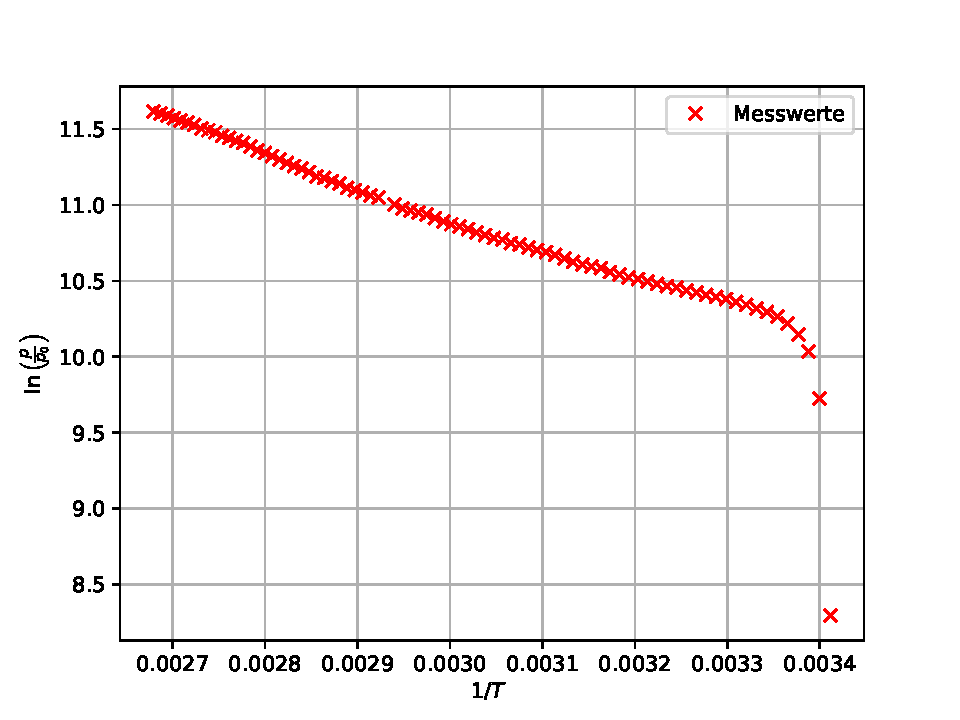
\includegraphics[height=6cm]{plota.pdf}  
    \caption{Bereich von $30$ bis $\SI{1000}{\milli\bar}$. $p_0=\SI{1}{\milli\bar}$.}
    \label{fig:MesswerteKlein}
  \end{subfigure}
  \hfill
  \begin{subfigure}{0.48\textwidth}
    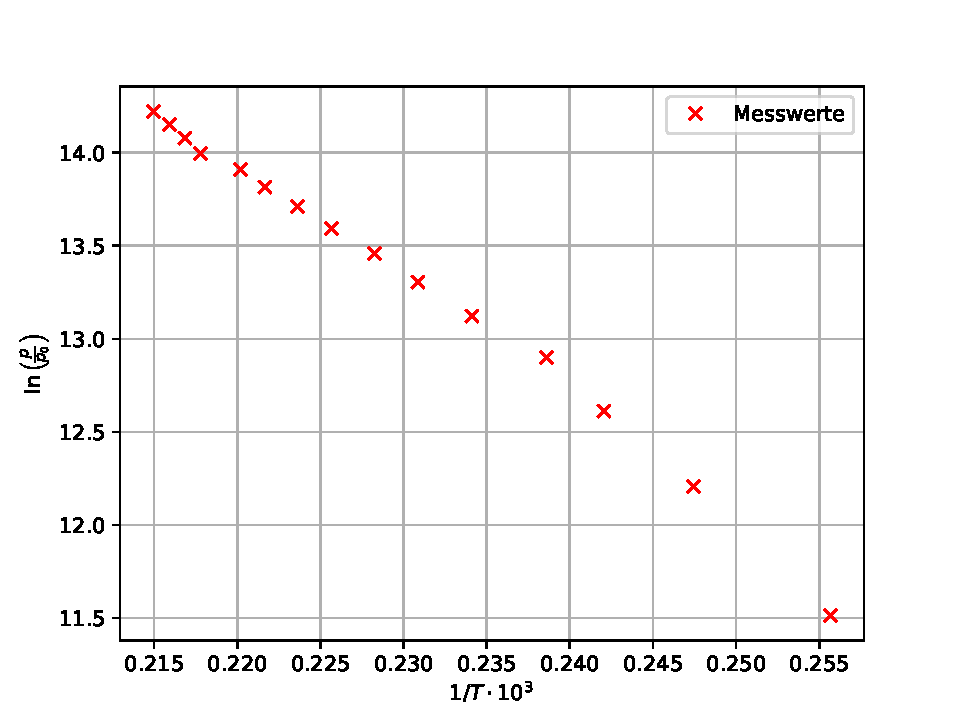
\includegraphics[height=6cm]{plotb.pdf}
    \caption{Bereich von $1$ bis $\SI{15}{\bar}$. $p_0=\SI{1}{\bar}$}
    \label{fig:MesswerteGross}
  \end{subfigure}
  \caption{Die Messwerte der ersten Messreihe aufgetragen als der Logarithmus des Drucks $p$
  gegen die reziproke absolute Temperatur $T$.}
  \label{fig:Teila}
\end{figure}
Um daraus die zu berechnende Verdampfungswärme des Wassers zu bestimmen, wird eine Gerade durch die Messwerte gelegt.
Diese wird mittels Python für den Bereich von $30$ bis $1000$\,mbar erstellt. \\
\begin{figure}[H]
  \centering
  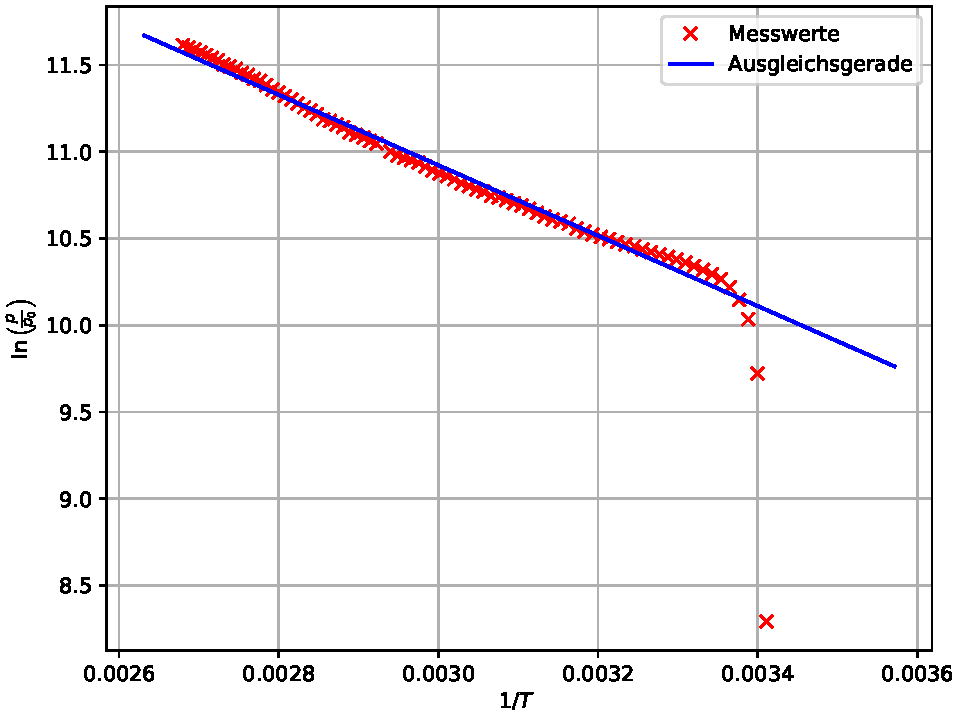
\includegraphics[scale=0.8]{plotc.pdf}
  \caption{Die Messwerte der zweiten Messreihe aufgetragen als der Logarithmus des Drucks $p$
  gegen die reziproke absolute Temperatur $T$ mit der Ausgleichsgerade. $p_0=1$\,mbar.}
  \label{fig:Ausgleichsgerade}
\end{figure}
Die Gleichung zur Bestimmung von $L$ und dem damit einhergehenden Fit ist wie folgt:
\begin{equation}
  ln(p) = - \frac{L}{R} \cdot \frac{1}{T}
  \Rightarrow y = a \cdot x + b = -2262 \cdot x + 17.69
\end{equation}
Mit numeric Python ergeben sich folgende Messunsicherheiten: $a = \SI{-2262 \pm 106 }{\frac{1}{\kelvin}}$
und $b = \SI{17.69 \pm 0.32}{\frac{1}{\kelvin}}$.
Die Verdampfungswärme wird mit folgendem Wert berechnet:
\begin{equation*}
  L = - \ a \cdot R \Rightarrow L = \SI{1.88 +- 0.09e4}{\frac{\J}{\mol}}
\end{equation*}
L ist die Steigung der Ausgleichsgeraden in Abbildung \ref{fig:Ausgleichsgerade} multipliziert mit der Universellen Gaskonstante R.
\noindent
Jetzt soll die äußere Verdampfungswärme $L_a$ bestimmt werden.
Diese beschreibt die benötigte Arbeit, um bei konstantem Druck das Volumen eines Stoffs zu verändern.
Hierfür wird die ideale Gasgleichung verwendet, die für ideale Gase genau diese Arbeit angibt.
\begin{equation}
    P \cdot V = R \cdot T = L_a
\end{equation}
Also ergibt sich $L_a = \SI{3101.3}{\frac{\J}{\mol}}$.
Um die erforderliche Arbeit zur Überwindung der molekularen Anziehungskraft bei Verdampfung $L_i$ zu bestimmen, wird
zunächst die Differenz zwischen $L$ und $L_a$ gebildet.
\begin{equation}
    L_i = L - L_a \Rightarrow L_i = \SI{15698.7 \pm 881.3}{\frac{\J}{\mol}}
\end{equation}
Um hier raus jetzt die Kraft für ein Molekül auszurechnen, muss die Definition für ein Mol eingesetzt werden.
Also muss $L_i$ durch die Avogadro-Konstante $N_a = \SI{6.022e23}{\per\mol}$ \cite{Avogadro} geteilt werden.
Zuletzt muss noch die Einheit in eV umgerechnet werden.
\begin{equation*}
  L_i = \SI{0.162722 \pm 0.009134 }{eV}
\end{equation*}

\subsection{Druck über einem Bar}
Auflösen der Clausius-Clapeyronschen Gleichung nach $L$ zur Bestimmung der Wärmeabhängigkeit ergibt.\\
\begin{align}
  &(V_D-V_F)dp=\frac{L}{T}dT\nonumber\\
  \Leftrightarrow L=&(V_D-V_F)\frac{dp}{dT}T\label{eqn:L(V,T)}
\end{align}
Mittels Python und scipy wird polynomialer Fit dritten Grades errechnet. Die 
zum Polynom $p(T)=a\cdot T^3+b\cdot T^2+c\cdot T+d$ gehörenen Vorfaktoren sind:
\begin{align*}
  a &= \num{2.1(0.6)e-5}\,\si{\bar\per\kelvin\cubed}\\
  b &= (-0.02 ± 0.008)\,\si{\bar\per\kelvin\squared}\\
  c &= (9.9 ± 3.3)\,\si{\bar\per\kelvin}\\
  d &= \num{-1.33(0.47)e3}\,\si{\pascal}\\
\end{align*}
\begin{figure}[H]
\centering
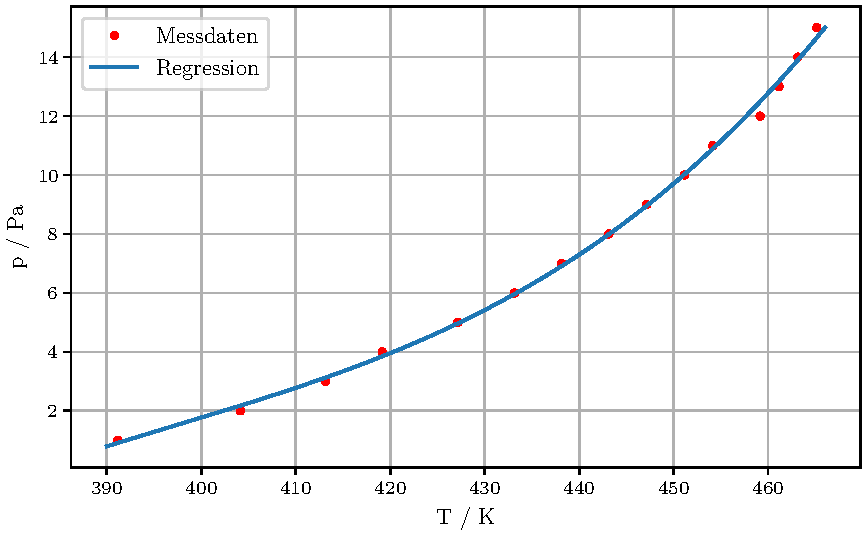
\includegraphics[height=7cm]{plotd.pdf}
\caption{Druck und Temperatur der zweiten Messreihe, $p\geq 1$Bar, sowie 
der Fit durch die Messwerte.}
\label{fig:Druck_groß}
\end{figure}
Ableitung des Polynoms $p(T)$ ergibt
\begin{equation}
p'(T)=3\cdot a\cdot T^2+2\cdot b\cdot T+c.
\end{equation}
Das ist der Asudruck für $\frac{dp}{dT}$.\\
In der Theorie wurde unter einer Bedingung die Annahme getroffen, dass $V_F$ gegen $V_D$
vernachlässigt werden darf. Dies wird hier genutzt. Nach umstellen der Formel aus der Theorie ergibt sich für $V=V_D$:
\begin{align}
   RT&=\left(p+\frac{a}{V^2}\right)V\\
   a\text{ ist hierbei } \text{gleich } &0,9\,\text{J m}^3\text{mol}^{-2}.\nonumber
   \intertext{Mithilfe der pq-Formel ergibt sich}
   \Rightarrow V&=\frac{RT}{2p}\pm\sqrt{\left(\frac{RT}{2p}\right)^2+\frac{a}{p}}\label{eqn:V(T)}
   \intertext{Durch einsetzen von Gl.\eqref{eqn:V(T)} in Gl.\eqref{eqn:L(V,T)} lässt sich folgender Ausdruck für L finden:}
   L(T)&=\frac{T}{P}\left(\frac{RT}{2}\pm\sqrt{\left(\frac{R^2T^2}{4}\right)-ap}\right).
\end{align}
Mit Python geplottet sieht $L(T)$ wie folgt aus:
\begin{figure}
  \begin{subfigure}{0.45\textwidth}
  \centering
  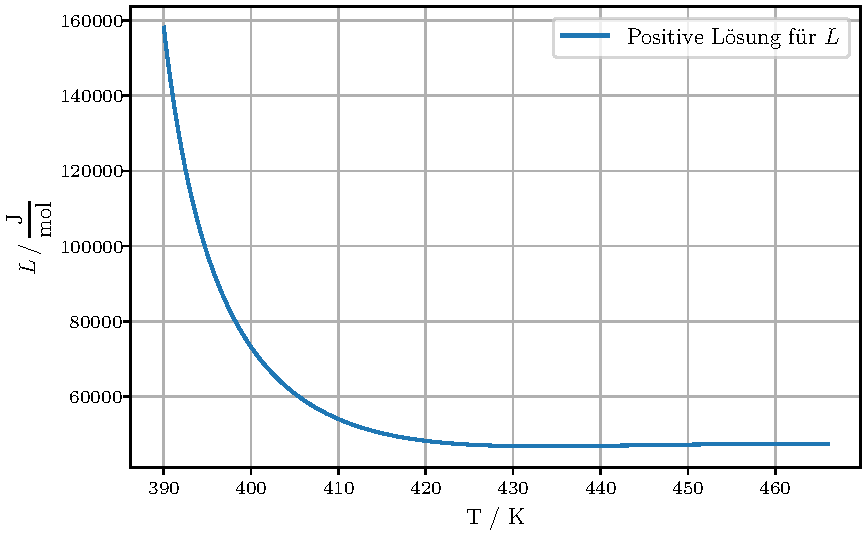
\includegraphics[height=4cm]{plote.pdf}
  \caption{$L$ in Abhängigkeit von T für $V_{D+}$.}
  \label{fig:Verdampfungswärme1}
  \end{subfigure}
  \hfill
  \begin{subfigure}{0.45\textwidth}
  \centering
  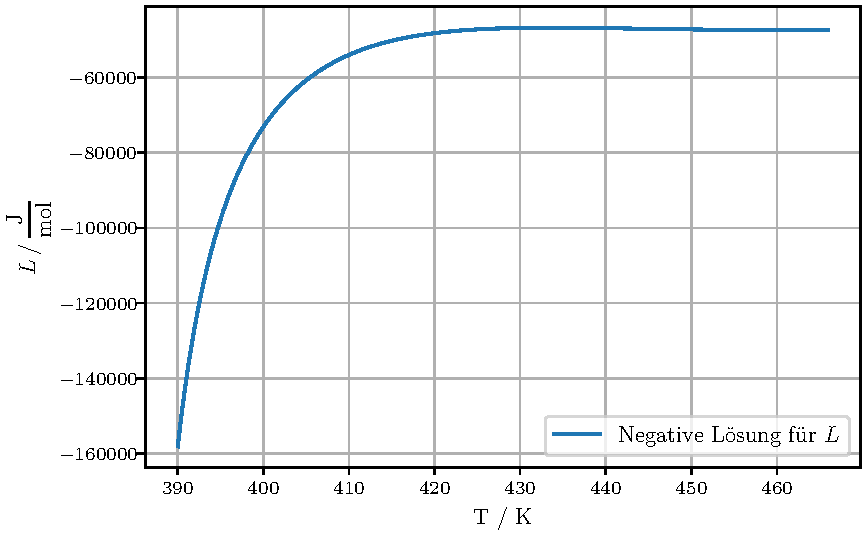
\includegraphics[height=4cm]{plotf.pdf}
  \caption{$L$ in Abhängigkeit von T für $V_{D-}$.}
  \label{fig:Verdampfungswärme2}
  \end{subfigure}
\end{figure}
